\chapter{Связь обобщенной модели Изинга с теорией чисел, теорией графов и комбинаторикой}\label{ch:ch5}

\section{Математические сечения и целочисленные последовательности в одномерной обобщенной модели Изинга}

Как уже отмечено, некоторые значения нуль-температурных энтропий и нуль-температурных намагниченностей выражаются через сечения, хорошо известные в теории чисел, а именно, через золотое сечение $\varphi$, серебряное сечение $\delta$, сверхзолотое сечение $\psi$, пластическое число $\rho$ и другие. Чтобы объяснить такое удивительное появление весьма большого количества математических констант при рассмотрении модели Изинга, стоит обратиться к важной теореме Фробениуса--Перрона. Эта теорема утверждает, что квадратная матрица со строго положительными вещественными элементами имеет одно наибольшее собственное значение, которое обязательно является вещественным и строго положительным. Кроме того, известно, что это наибольшее собственное значение является так называемым \emph{числом Перрона}. Это означает, что искомое собственное значение уравнения является вещественным и больше единицы, при этом все сопряженные корни уравнения меньше искомого собственного значения по абсолютной величине. 

Поскольку аргумент натурального логарифма в выражениях для нуль-температурной энтропии является статистическим весом системы $\Omega$, то эта величина может принимать значение только в промежутке $1\leqslant \Omega\leqslant 2$. Откуда следует, что $S= \ln \Omega =  \ln 1 = 0$ (при $T \rightarrow 0$), что в результате соответствует ситуациям, при которых система обладает лишь одной конфигурацией (фрустрации отсутствуют). Поэтому все остальные найденные значения статистического веса (при $T \rightarrow 0$), выраженные через $\varphi$, $\rho$, $\psi$,  $\sqrt{2}$ и другие математические сечения, в том числе и новые (безымянные), приходящегося на один узел цепочки, помимо того, что они являются числами Перрона~\cite{wu2010, lind1992, boyd1985}, соответствуют определенным фрустрирующим состояниям системы, т.е. в основном состоянии наблюдается бесконечно много конфигураций, в том числе и без какой-либо трансляционной инвариантности. Следует отметить, что в модели Изинга энтропия достигает своего максимального значения $\ln 2$ в двух случаях: 1. При стремлении температуры к бесконечности, при которой статистические веса всех $2^N$ конфигураций при любых значениях обменных интегралов совпадают. 2. В парамагнетике, в котором все обменные интегралы равны нулю, статистические веса всех $2^N$ конфигураций совпадают при любой температуре, так что энтропия равна $\ln 2$ при всех температурах, и фактически парамагнетик является абсолютно фрустрированной системой, что впервые отмечено в работе~\cite{zarubin2019}. 

Можно показать, что фрустрирующее значение нуль-температурной энтропии определяется как предел некоторой последовательности в следующем виде
\begin{equation}
S_{\text{fr}}=\lim_{N\rightarrow \infty} \ln \bigg[\frac{\widetilde{Z}_{N+1}}{\widetilde{Z}_N}\bigg],
\label{41}
\end{equation}
где $\widetilde{Z}_{N+1}$ --- число допустимых конфигураций в основном состоянии для $N+1$ узлов, $\widetilde{Z}_N$ --- число допустимых конфигураций в основном состоянии для $N$ узлов.

Фрустрационную нуль-температурную намагниченность также можно найти как предел последовательности
\begin{equation}
M_{\text{fr}}=\lim_{N\rightarrow \infty}\frac{M_{\Sigma}}{\widetilde{Z}_N},
\label{42}
\end{equation}
где $M_{\Sigma}$ --- общая (суммарная) намагниченность всех допустимых конфигураций в основном состоянии.

Произведя подсчет возможных конфигураций $\widetilde{Z}_{N}$ для конкретного числа узлов $N$ для случая только ближайших соседей во внешнем магнитном поле, была определена последовательность
\[\widetilde{Z}_{N}^{\varphi} = 1, 3, 4, 7, 11, 18, 29, 47, 76, \dots\]  

Полученная последовательность чисел известна как \emph{последовательность Люка}, которая задается рекуррентным соотношением $a_n=a_{n-1}+a_{n-2}$ с начальными значениями $a_0 = 2$ и $a_1 = 1$. 

Как известно~\cite{sloane1973}--\cite{hoggatt1969}, отношение $\widetilde{Z}_{N+1}^{\varphi}/\widetilde{Z}_{N}^{\varphi}$ стремится к золотому сечению $\varphi$, а, следовательно, $\ln (\widetilde{Z}_{N+1}^{\varphi}/\widetilde{Z}_{N}^{\varphi})$ стремится к натуральному логарифму золотого сечения $\ln \varphi$.

В свою очередь, можно показать, что общая намагниченность для всех допустимых конфигураций в основном состоянии $M_{\Sigma}$ для случая только ближайших соседей во внешнем магнитном поле представлена последовательностью \emph{чисел Фибоначчи} c рекуррентным соотношением $a_n=a_{n-1}+a_{n-2}$, но с начальными условиями $a_0 = 0$ и $a_1 = 1$
\[M_{\Sigma}^{\varphi} = 1, 1, 2, 3, 5, 8 , 13, 21, 34, \dots\]

Взяв отношение последовательности Фибоначчи к последовательности Люка $M_{\Sigma}^{\varphi}/\widetilde{Z}_{N}^{\varphi}$ в термодинамическом пределе ($N\rightarrow \infty$), получим значение фрустрационной намагниченности равное $1/(2\varphi-1)$.

 \begin{figure}[h]
 	\begin{minipage}{0.49\linewidth}
 		\center{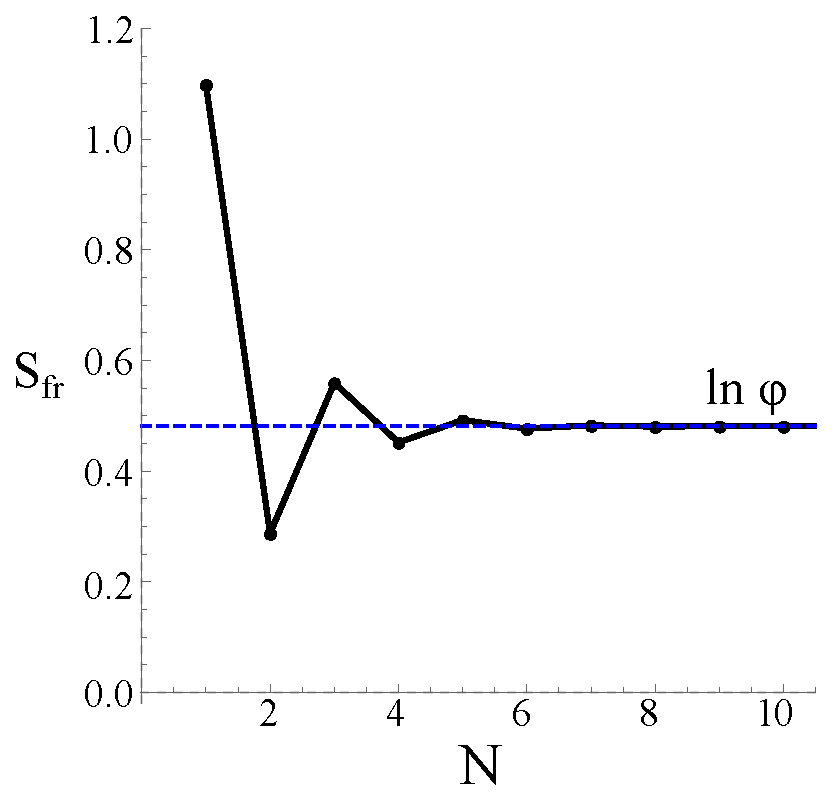
\includegraphics[width=0.85\linewidth]{part5/sfr.eps} \\ а)}
 	\end{minipage}
 	\hfill
 	\begin{minipage}{0.49\linewidth}
 		\center{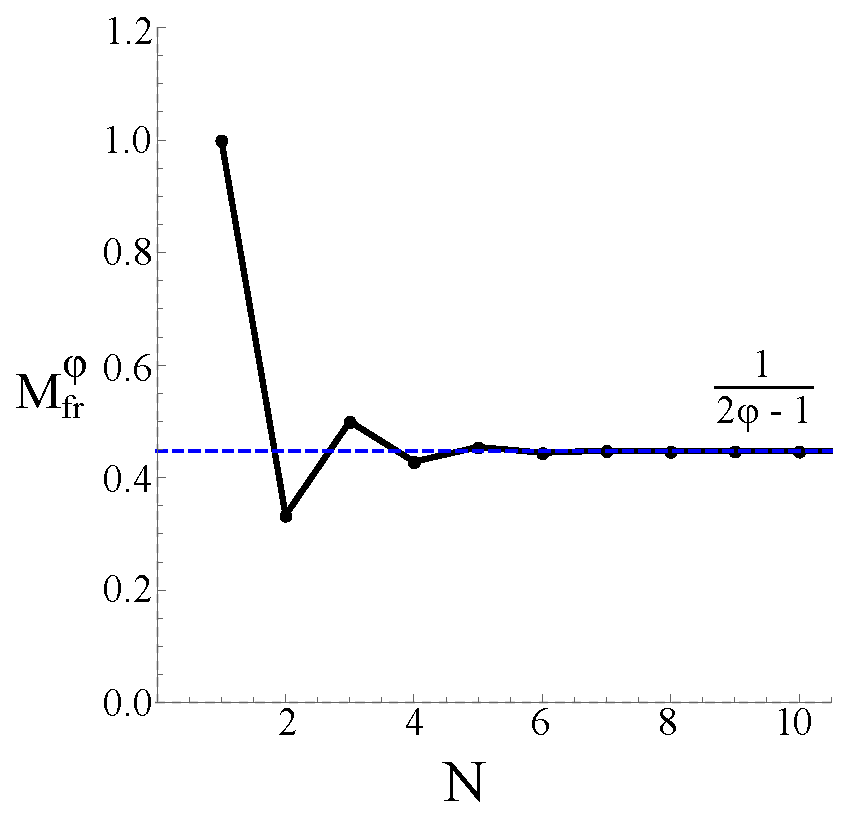
\includegraphics[width=0.85\linewidth]{part5/mfr.eps} \\ б)}
 	\end{minipage}
 	\caption{Наглядное представление сходимости а) последовательности $\ln (\widetilde{Z}_{N+1}^{\varphi}/\widetilde{Z}_{N}^{\varphi})$ к нуль-температурному значению энтропии равной $\ln \varphi$ и б) последовательности $M_{\Sigma}^{\varphi}/\widetilde{Z}_{N}^{\varphi}$ к нуль-температурному значению намагниченности равной $1/(2\varphi - 1)$}
 	\label{fr1}
 \end{figure}

В правильности полученных выше результатов можно убедиться, глядя на рисунок~\ref{fr1}. Видно, что последовательности $\ln (\widetilde{Z}_{N+1}^{\varphi}/\widetilde{Z}_{N}^{\varphi})$ и $M_{\Sigma}^{\varphi}/\widetilde{Z}_{N}^{\varphi}$ быстро сходятся к нуль-температурной энтропии равной $\ln \varphi$ и нуль-температурной намагниченности равной $1/(2\varphi - 1)$ соответственно.

Учитывая взаимодействия не только между ближайшими, но и между вторыми соседями в магнитном поле при антиферромагнитных взаимодействиях и тех и других, возникают два фрустрирующих поля. Значение нуль-температурной намагниченности в первом фрустрирующем поле выражается отношением некоторых последовательностей чисел, первая из которых определяется по правилу $a_n = a_{n-3} + a_{n-4}$ с начальными значениями $a_0 = 1$ и $a_1 = a_2 = a_3 = 1$
\[M^{\xi}_{\Sigma} = 0, 0, 0, 1, 0, 0, 1, 1, 0, 1, 2, 1, 1, 3, \dots\]
Вторая последовательность определяется по тому же правилу $a_n = a_{n-3} + a_{n-4}$, но с начальными значениями $a_0 = 4$, $a_1 = a_2 = 0$, $a_3 = 3$  \[\widetilde{Z}^{\xi}_{N} = 4, 0, 0, 3, 4, 0, 3, 7, 4, 3, 10, 11, 7, 13, \dots\]
Взяв отношение первой последовательности ко второй при $N\rightarrow \infty$ получим значение нуль-температурной намагниченности $1/(\xi+4\xi^3-\xi^4)$ с соответствующей энтропией равной $\ln \xi$.

Значение намагниченности во втором фрустрирующем поле представлено отношением \emph{последовательности коров Нараяны}~\cite{allouche1996, lin2021} c рекуррентным уравнением $a_n = a_{n-1} + a_{n-3}$ и начальными значениями $a_0 = a_1 = a_2 = 1$
\[M^{\psi}_{\Sigma} = 1, 1, 1 , 2, 3, 4, 6, 9, 13, 19, 28, \dots\] к последовательности c тем же рекуррентным уравнением, что и последовательность Нараяны, но с начальными значениями $a_0 = 3$, $a_1 = a_2 = 1$ \[\widetilde{Z}^{\psi}_{N} = 3, 1, 1, 4, 5, 6, 10, 15, 21, \dots\] Отметим, что приведенная последовательность $\widetilde{Z}^{\psi}_{N}$ до сих пор не изучена. 
Отношение данных последовательностей при $N\rightarrow \infty$ дает значение нуль-температурной намагниченности $\psi^3/(\psi^2+3)$, а соответствующая энтропия равна натуральному логарифму сверхзолотого сечения $\ln \psi$. Сходимости последовательностей проиллюстрированы на рисунке~\ref{fr2}.

 \begin{figure}[h]
 	\begin{minipage}{0.49\linewidth}
 		\center{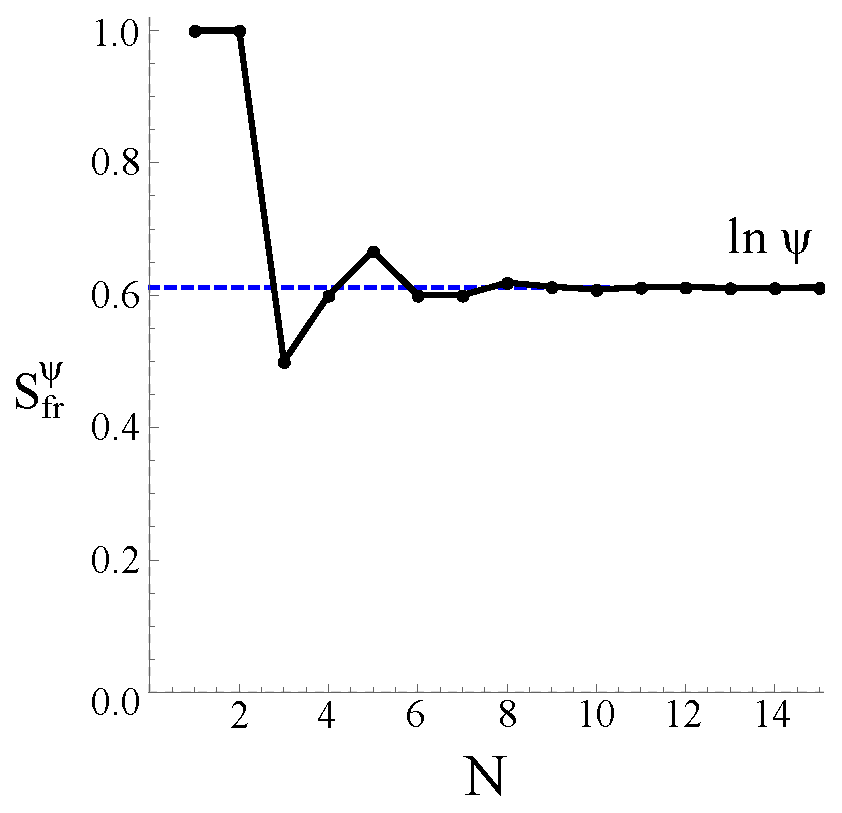
\includegraphics[width=0.85\linewidth]{part5/sfr1.eps} \\ а)}
 	\end{minipage}
 	\hfill
 	\begin{minipage}{0.49\linewidth}
 		\center{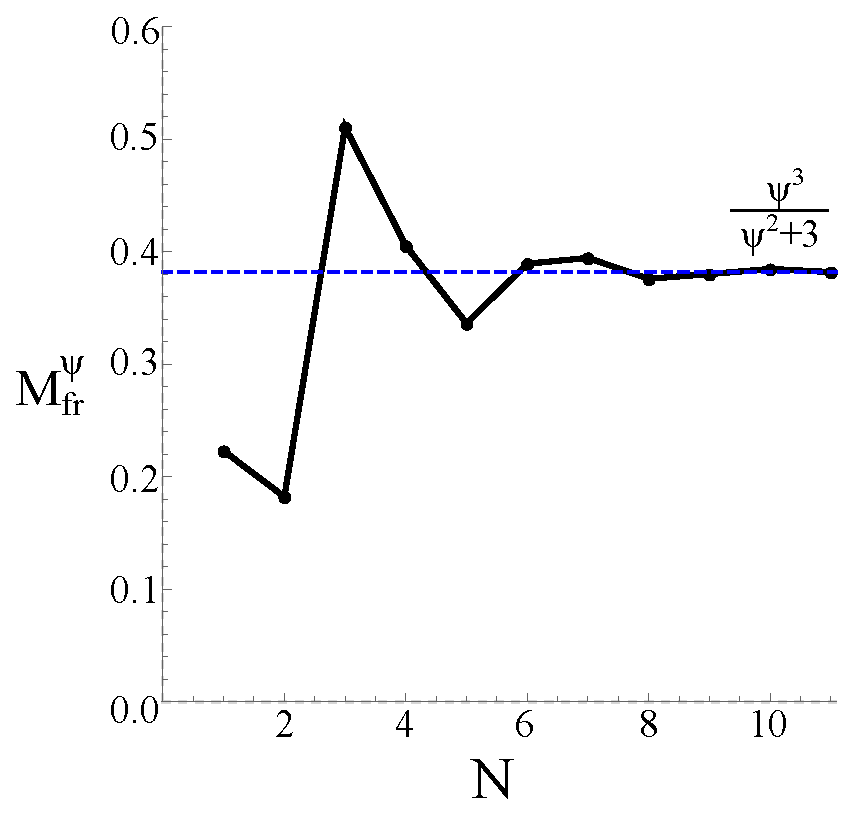
\includegraphics[width=0.85\linewidth]{part5/mfr1.eps} \\ б)}
 	\end{minipage}
 	\caption{Наглядное представление сходимости а) последовательности $\ln (\widetilde{Z}_{N+1}^{\psi}/\widetilde{Z}_{N}^{\psi})$ к нуль-температурному значению энтропии равной $\ln \psi$ и б) последовательности $M_{\Sigma}^{\psi}/\widetilde{Z}_{N}^{\psi}$ к нуль-температурному значению намагниченности равной $\psi^3/(\psi^2+3)$}
 	\label{fr2}
 \end{figure}

При ферромагнитных взаимодействиях ближайших соседей и антиферромагнитных взаимодействиях вторых соседей, намагниченность равна отношению последовательности, задаваемой рекуррентным уравнением $a_n = a_{n-1} + a_{n-4}$ с начальными значениями $a_0 = 0$, $a_1 = a_2 = a_3 = 1$ \[M^{\mu}_{\Sigma} = 0, 1, 1, 1, 1, 2, 3, 4, 5, 7, 10, 14, 19, 26 \dots\] к последовательности c тем же рекуррентным уравнением $a_n = a_{n-1} + a_{n-4}$, но с начальными значениями $a_0 = 4$, $a_1 = a_2 = a_3 = 1$ \[\widetilde{Z}^{\mu}_{N} = 4, 1, 1, 1, 5, 6, 7, 8, 13, \dots\] 

Обратим внимание на то, что последовательность $\widetilde{Z}^{\mu}_{N}$ также до настоящего момента не была исследована.
При $N\rightarrow \infty$ отношение последовательностей дает значение нуль-температурной намагниченности $\mu^4/(\mu^3+4\mu+1)$ с энтропией равной $\ln \mu$.

Другие значения нуль-температурных энтропий и нуль-температурных намагниченностей, представленные в данной работе, могут быть представлены через пределы последовательностей (также известных из математики~\cite{sloane1973, sloane1995}, \cite{bicknell1975, vieira2020, adams1982}) только с помощью формул \eqref{41} и \eqref{42} без привлечения формализма трансфер-матрицы Крамерса--Ваннье. Однако, многие из встречаемых последовательностей являются неизученными.

Таким образом установлено, что фрустрационные свойства модели Изинга тесным образом связаны с достижениями в теории чисел, известными уже на протяжении столетий.

\section{Замощение шахматной решетки плитками домино}

Помимо классических подходов к решению двумерной модели Изинга, таких как точное аналитическое решение Онзагера и комбинаторные методы, существует альтернативный и весьма мощный метод, известный как метод димеров. Этот метод был существенно развит в работах Кастелайна~\cite{kasteleyn1961, kasteleyn1963_1, kasteleyn1963_2}, Темперли~\cite{temperley1961} и Фишера~\cite{fisher1966}.

Димер — это ребро графа, которое покрывает ровно две соседние вершины. Задача подсчета числа димерных покрытий графа, то есть разбиений множества вершин графа на пары, связанных ребрами, является классической в комбинаторике и статистической механике. Она тесно связана с изучением различных моделей взаимодействующих систем.

Идея применения димерных покрытий к решению модели Изинга возникла из наблюдения, что конфигурации спинов в модели Изинга можно однозначно сопоставить с определенными димерными покрытиями специально построенного графа. Для двумерной модели Изинга на квадратной решетке существует соответствие между конфигурациями спинов и димерными покрытиями некоторого связанного графа, что позволяет свести задачу вычисления статистической суммы модели Изинга к задаче подсчета числа димерных покрытий.

В начале 1960-х годов Кастелайн разработал метод вычисления числа димерных покрытий плоских графов, введя понятие так называемой ориентации Кастелайна. Эта ориентация представляет собой направление ребер графа, обладающее особым свойством: для каждого цикла нечетной длины число ребер, ориентированных в определенном направлении, должно быть нечетным. Благодаря такой ориентации задача подсчета числа димерных покрытий сводится к вычислению определителя специально построенной матрицы смежности графа, что значительно упрощает вычисления.

Независимо от Кастелайна, Фишер совместно с Темперли разработали методы, позволяющие выразить статистическую сумму модели Изинга через задачи подсчета димерных покрытий. Фишер предложил конструкцию, которая переводит исходную задачу Изинга в задачу димеров на так называемом расширенном графе (Fisher graph). В этом графе вершины и ребра модифицированы таким образом, чтобы сохранить всю информацию об исходной модели, что дает возможность применить методы подсчета димерных покрытий к вычислению статистической суммы.

Таким образом, метод димеров является еще одним способом получения точного аналитического решения двумерной модели Изинга.

Важным связным понятием является задача замощения квадратной решетки плитками домино (domino tiling). Эта задача формулируется как поиск числа всех возможных способов покрытия квадратной решетки плитками размером $2 \times 1$, без наложений и пропусков. Эта задача эквивалентна подсчету совершенных паросочетаний на графе, где каждая вершина соответствует ячейке решетки, а ребро — смежности ячеек. Несмотря на кажущуюся простоту, задача является нетривиальной и была независимо решена в 1960-х годах классиками теории графов и статистической механики — Кастелайном~\cite{kasteleyn1961} и совместно Темперли с Фишером~\cite{temperley1961}.

Из этих работ можно выделить два ключевых результата. Во-первых, формула Кастелайна для подсчета числа замощений квадратной решетки плитками домино (или числа совершенных паросочетаний графа)~\cite{kasteleyn1961}. Эта формула корректно работает для решеток с четным числом квадратов по обеим сторонам ($m$ и $n$). При нечетных значениях $m$ или $n$ число замощений равно нулю, что интуитивно понятно — решетку с нечетным количеством ячеек невозможно полностью покрыть плитками размером $2 \times 1$. Во-вторых, было получено асимптотическое выражение для числа замощений при стремлении размеров решетки к бесконечности. Поскольку абсолютное количество замощений экспоненциально растет с увеличением площади решетки, полезнее рассматривать количество замощений на одну плитку домино (или один димер). Это значение было найдено авторами независимо и оказалось равным $\exp (2G/\pi)$, где $G$ — постоянная Каталана.

Возвращаясь к данной работе, следует подчеркнуть, что предложенная Сиози~\cite{syozi1972} решетка, являющаяся обобщением квадратной решетки с произвольным числом трансляций в горизонтальном и вертикальном направлениях, в своем простейшем случае может быть преобразована в так называемую <<шахматную решетку>>, обладающую двумя трансляциями в каждом из направлений. Именно такую структуру и исследует данная работа.

По сути, Кастелайн и другие исследователи в своих работах анализировали именно шахматную решетку, поскольку каждый димер в такой решетке покрывает пару соседних узлов разных типов. В настоящей работе эти два типа узлов обозначены символами кружка ($\circ$) и крестика ($\times$)~(см. рис.~\ref{point}).

В рамках проведенного исследования получено значение нуль-температурной энтропии на один спин обобщённой квадратной решётки с двумя трансляциями, равное $G/\pi$. Кроме того, обнаружено еще одно значение нуль-температурной энтропии, равное $1/(2\pi)\Cl_2(\pi/3)$, что ровно в два раза меньше, чем значение нуль-температурной энтропии, найденное Ваннье для треугольной решетки~\cite{wannier1950}, равное $\Cl_2(\pi/3) = 0.3230\dots$.

Все эти факты указывают на глубокую связь между значениями фрустрационной энтропии в модели Изинга и задачей замощения решетки плитками домино. Однако, данный тезис требует дальнейшей проверки и более тщательного теоретического обоснования.

\section{Выводы по главе}

В одномерной модели Изинга значения нуль-температурных энтропий и намагниченностей выражаются через пределы некоторых целочисленных последовательностей, не  прибегая к формализму трансфер-матрицы.

Важным результатом является выявление двух фундаментальных значений нуль-температурной энтропии, связанных со специальными математическими константами — постоянной Каталана и функцией Клаузена. Эти значения отражают глубокую связь фрустраций в модели Изинга с комбинаторными задачами, такими как замощение решетки плитками домино.

Установлена тесная связь между фрустрационной энтропией обобщенной модели Изинга и классической задачей подсчета димерных покрытий (замощений плитками домино), что открывает перспективы для дальнейших исследований, объединяющих методы статистической физики, комбинаторики и теории графов.

Результаты, описанные в этой главе, опубликованы автором в работе~\cite{vakbib3}.

\FloatBarrier